% Options for packages loaded elsewhere
\PassOptionsToPackage{unicode}{hyperref}
\PassOptionsToPackage{hyphens}{url}
%
\documentclass[
  ignorenonframetext,
]{beamer}
\usepackage{pgfpages}
\setbeamertemplate{caption}[numbered]
\setbeamertemplate{caption label separator}{: }
\setbeamercolor{caption name}{fg=normal text.fg}
\beamertemplatenavigationsymbolsempty
% Prevent slide breaks in the middle of a paragraph
\widowpenalties 1 10000
\raggedbottom
\setbeamertemplate{part page}{
  \centering
  \begin{beamercolorbox}[sep=16pt,center]{part title}
    \usebeamerfont{part title}\insertpart\par
  \end{beamercolorbox}
}
\setbeamertemplate{section page}{
  \centering
  \begin{beamercolorbox}[sep=12pt,center]{part title}
    \usebeamerfont{section title}\insertsection\par
  \end{beamercolorbox}
}
\setbeamertemplate{subsection page}{
  \centering
  \begin{beamercolorbox}[sep=8pt,center]{part title}
    \usebeamerfont{subsection title}\insertsubsection\par
  \end{beamercolorbox}
}
\AtBeginPart{
  \frame{\partpage}
}
\AtBeginSection{
  \ifbibliography
  \else
    \frame{\sectionpage}
  \fi
}
\AtBeginSubsection{
  \frame{\subsectionpage}
}
\usepackage{amsmath,amssymb}
\usepackage{lmodern}
\usepackage{ifxetex,ifluatex}
\ifnum 0\ifxetex 1\fi\ifluatex 1\fi=0 % if pdftex
  \usepackage[T1]{fontenc}
  \usepackage[utf8]{inputenc}
  \usepackage{textcomp} % provide euro and other symbols
\else % if luatex or xetex
  \usepackage{unicode-math}
  \defaultfontfeatures{Scale=MatchLowercase}
  \defaultfontfeatures[\rmfamily]{Ligatures=TeX,Scale=1}
  \setmainfont[BoldFont = SF Pro Rounded Semibold]{SF Pro Rounded}
  \setmathfont[]{STIX Two Math}
\fi
\usefonttheme{serif} % use mainfont rather than sansfont for slide text
% Use upquote if available, for straight quotes in verbatim environments
\IfFileExists{upquote.sty}{\usepackage{upquote}}{}
\IfFileExists{microtype.sty}{% use microtype if available
  \usepackage[]{microtype}
  \UseMicrotypeSet[protrusion]{basicmath} % disable protrusion for tt fonts
}{}
\makeatletter
\@ifundefined{KOMAClassName}{% if non-KOMA class
  \IfFileExists{parskip.sty}{%
    \usepackage{parskip}
  }{% else
    \setlength{\parindent}{0pt}
    \setlength{\parskip}{6pt plus 2pt minus 1pt}}
}{% if KOMA class
  \KOMAoptions{parskip=half}}
\makeatother
\usepackage{xcolor}
\IfFileExists{xurl.sty}{\usepackage{xurl}}{} % add URL line breaks if available
\IfFileExists{bookmark.sty}{\usepackage{bookmark}}{\usepackage{hyperref}}
\hypersetup{
  pdftitle={444 Lecture 2.8 - Ice Cream},
  pdfauthor={Brian Weatherson},
  hidelinks,
  pdfcreator={LaTeX via pandoc}}
\urlstyle{same} % disable monospaced font for URLs
\newif\ifbibliography
\usepackage{graphicx}
\makeatletter
\def\maxwidth{\ifdim\Gin@nat@width>\linewidth\linewidth\else\Gin@nat@width\fi}
\def\maxheight{\ifdim\Gin@nat@height>\textheight\textheight\else\Gin@nat@height\fi}
\makeatother
% Scale images if necessary, so that they will not overflow the page
% margins by default, and it is still possible to overwrite the defaults
% using explicit options in \includegraphics[width, height, ...]{}
\setkeys{Gin}{width=\maxwidth,height=\maxheight,keepaspectratio}
% Set default figure placement to htbp
\makeatletter
\def\fps@figure{htbp}
\makeatother
\setlength{\emergencystretch}{3em} % prevent overfull lines
\providecommand{\tightlist}{%
  \setlength{\itemsep}{0pt}\setlength{\parskip}{0pt}}
\setcounter{secnumdepth}{-\maxdimen} % remove section numbering
\let\Tiny=\tiny

 \setbeamertemplate{navigation symbols}{} 

% \usetheme{Madrid}
 \usetheme[numbering=none, progressbar=foot]{metropolis}
 \usecolortheme{wolverine}
 \usepackage{color}
 \usepackage{MnSymbol}
% \usepackage{movie15}

\usepackage{amssymb}% http://ctan.org/pkg/amssymb
\usepackage{pifont}% http://ctan.org/pkg/pifont
\newcommand{\cmark}{\ding{51}}%
\newcommand{\xmark}{\ding{55}}%

\DeclareSymbolFont{symbolsC}{U}{txsyc}{m}{n}
\DeclareMathSymbol{\boxright}{\mathrel}{symbolsC}{128}
\DeclareMathAlphabet{\mathpzc}{OT1}{pzc}{m}{it}

\setlength{\parskip}{1ex plus 0.5ex minus 0.2ex}

\AtBeginSection[]
{
\begin{frame}
	\Huge{\color{darkblue} \insertsection}
\end{frame}
}

\renewenvironment*{quote}	
	{\list{}{\rightmargin   \leftmargin} \item } 	
	{\endlist }

\definecolor{darkgreen}{rgb}{0,0.7,0}
\definecolor{darkblue}{rgb}{0,0,0.8}

\usepackage[italic]{mathastext}
\usepackage{nicefrac}

\setbeamertemplate{caption}{\raggedright\insertcaption}

%\def\toprule{}
%\def\bottomrule{}
%\def\midrule{}
\usepackage{etoolbox}
\AfterEndEnvironment{description}{\vspace{9pt}}
\AfterEndEnvironment{oltableau}{\vspace{9pt}}
\BeforeBeginEnvironment{oltableau}{\vspace{9pt}}
\AfterEndEnvironment{center}{\vspace{9pt}}
\BeforeBeginEnvironment{tabular}{\vspace{9pt}}
\AfterEndEnvironment{longtable}{\vspace{-6pt}}
\usepackage{booktabs}
\usepackage{longtable}
\usepackage{array}
\usepackage{multirow}
\usepackage{wrapfig}
\usepackage{float}
\usepackage{colortbl}
\usepackage{pdflscape}
\usepackage{tabu}
\usepackage{threeparttable} 
\usepackage{threeparttablex} 
\usepackage[normalem]{ulem} 
\usepackage{makecell}
\usepackage{xcolor}
\usepackage{ulem}

\setlength\heavyrulewidth{0ex}
\setlength\lightrulewidth{0.08ex}

\aboverulesep=0ex
\belowrulesep=0ex
\renewcommand{\arraystretch}{1.2}
\ifluatex
  \usepackage{selnolig}  % disable illegal ligatures
\fi

\title{444 Lecture 2.8 - Ice Cream}
\author{Brian Weatherson}
\date{}

\begin{document}
\frame{\titlepage}

\begin{frame}{Plan}
\protect\hypertarget{plan}{}
To look at a famous example of iterated deletion.
\end{frame}

\begin{frame}{Reading}
\protect\hypertarget{reading}{}
This isn't in the book.
\end{frame}

\begin{frame}{Example}
\protect\hypertarget{example}{}
Two trucks have to choose where they will sell ice-cream on a particular
beach. There are 7 locations to choose from, which we'll number 0, 1,
\ldots, 5, 6. Spot 0 is at the left end of the beach, Spot 6 is at the
right end of the beach, and the other spots are equally spaced in
between. There are 10 people at each location. Each of them will buy
ice-cream. If one truck is closer, they will buy ice-cream from that
truck. If two trucks are equally close, then 5 of them will buy
ice-cream from one truck, and 5 from the other. Each truck aims to
maximise the amount of ice-cream it sells. Where should the trucks end
up?
\end{frame}

\begin{frame}
\begin{table}[!h]
\centering
\begin{tabular}[t]{>{}r|ccccccc}
\toprule
 & 0 & 1 & 2 & 3 & 4 & 5 & 6\\
\midrule
0 & 35, 35 & 10, 60 & 15, 55 & 20, 50 & 25, 45 & 30, 40 & 35, 35\\
1 & 60, 10 & 35, 35 & 20, 50 & 25, 45 & 30, 40 & 35, 35 & 40, 30\\
2 & 55, 15 & 50, 20 & 35, 35 & 30, 40 & 35, 35 & 40, 30 & 45, 25\\
3 & 50, 20 & 45, 25 & 40, 30 & 35, 35 & 40, 30 & 45, 25 & 50, 20\\
4 & 45, 25 & 40, 30 & 35, 35 & 30, 40 & 35, 35 & 50, 20 & 55, 15\\
5 & 40, 30 & 35, 35 & 30, 40 & 25, 55 & 20, 50 & 35, 35 & 60, 10\\
6 & 35, 35 & 30, 40 & 25, 45 & 20, 50 & 15, 55 & 10, 60 & 35, 35\\
\bottomrule
\end{tabular}
\end{table}

\begin{itemize}
\tightlist
\item
  Think about why each of these payoffs is correct.
\end{itemize}
\end{frame}

\begin{frame}
\begin{table}[!h]
\centering
\begin{tabular}[t]{>{}r|ccccccc}
\toprule
 & 0 & 1 & 2 & 3 & 4 & 5 & 6\\
\midrule
0 & \textcolor{red}{35}, 35 & \textcolor{red}{10}, 60 & \textcolor{red}{15}, 55 & \textcolor{red}{20}, 50 & \textcolor{red}{25}, 45 & \textcolor{red}{30}, 40 & \textcolor{red}{35}, 35\\
1 & \textcolor{darkgreen}{60}, 10 & \textcolor{darkgreen}{35}, 35 & \textcolor{darkgreen}{20}, 50 & \textcolor{darkgreen}{25}, 45 & \textcolor{darkgreen}{30}, 40 & \textcolor{darkgreen}{35}, 35 & \textcolor{darkgreen}{40}, 30\\
2 & 55, 15 & 50, 20 & 35, 35 & 30, 40 & 35, 35 & 40, 30 & 45, 25\\
3 & 50, 20 & 45, 25 & 40, 30 & 35, 35 & 40, 30 & 45, 25 & 50, 20\\
4 & 45, 25 & 40, 30 & 35, 35 & 30, 40 & 35, 35 & 50, 20 & 55, 15\\
5 & 40, 30 & 35, 35 & 30, 40 & 25, 55 & 20, 50 & 35, 35 & 60, 10\\
6 & 35, 35 & 30, 40 & 25, 45 & 20, 50 & 15, 55 & 10, 60 & 35, 35\\
\bottomrule
\end{tabular}
\end{table}

\begin{itemize}
\tightlist
\item
  I've highlighted Row's payoffs for 0 and 1 to make it clear that 1
  strongly dominates 0.
\end{itemize}
\end{frame}

\begin{frame}
\begin{table}[!h]
\centering
\begin{tabular}[t]{>{}r|ccccccc}
\toprule
 & 0 & 1 & 2 & 3 & 4 & 5 & 6\\
\midrule
0 & 35, 35 & 10, 60 & 15, 55 & 20, 50 & 25, 45 & 30, 40 & 35, 35\\
1 & 60, 10 & 35, 35 & 20, 50 & 25, 45 & 30, 40 & 35, 35 & 40, 30\\
2 & 55, 15 & 50, 20 & 35, 35 & 30, 40 & 35, 35 & 40, 30 & 45, 25\\
3 & 50, 20 & 45, 25 & 40, 30 & 35, 35 & 40, 30 & 45, 25 & 50, 20\\
4 & 45, 25 & 40, 30 & 35, 35 & 30, 40 & 35, 35 & 50, 20 & 55, 15\\
5 & 40, 30 & 35, 35 & 30, 40 & 25, 55 & 20, 50 & 35, 35 & 60, 10\\
6 & 35, 35 & 30, 40 & 25, 45 & 20, 50 & 15, 55 & 10, 60 & 35, 35\\
\bottomrule
\end{tabular}
\end{table}

\begin{itemize}
\tightlist
\item
  But 2 doesn't dominate 1, because 1 is a better response to 0 than 2
  is.
\end{itemize}
\end{frame}

\begin{frame}
\begin{table}[!h]
\centering
\begin{tabular}[t]{>{}r|ccccccc}
\toprule
 & 0 & 1 & 2 & 3 & 4 & 5 & 6\\
\midrule
0 & 35, 35 & 10, 60 & 15, 55 & 20, 50 & 25, 45 & 30, 40 & 35, 35\\
1 & 60, 10 & 35, 35 & 20, 50 & 25, 45 & 30, 40 & 35, 35 & 40, 30\\
2 & 55, 15 & 50, 20 & 35, 35 & 30, 40 & 35, 35 & 40, 30 & 45, 25\\
3 & 50, 20 & 45, 25 & 40, 30 & 35, 35 & 40, 30 & 45, 25 & 50, 20\\
4 & 45, 25 & 40, 30 & 35, 35 & 30, 40 & 35, 35 & 50, 20 & 55, 15\\
5 & 40, 30 & 35, 35 & 30, 40 & 25, 55 & 20, 50 & 35, 35 & 60, 10\\
6 & 35, 35 & 30, 40 & 25, 45 & 20, 50 & 15, 55 & 10, 60 & 35, 35\\
\bottomrule
\end{tabular}
\end{table}

\begin{itemize}
\tightlist
\item
  The game is symmetric around 3, so 5 also dominates 6 (and is not
  dominated by 4).
\end{itemize}
\end{frame}

\begin{frame}
\begin{table}[!h]
\centering
\begin{tabular}[t]{>{}r|ccccccc}
\toprule
 & 0 & 1 & 2 & 3 & 4 & 5 & 6\\
\midrule
0 & 35, 35 & 10, 60 & 15, 55 & 20, 50 & 25, 45 & 30, 40 & 35, 35\\
1 & 60, 10 & 35, 35 & 20, 50 & 25, 45 & 30, 40 & 35, 35 & 40, 30\\
2 & 55, 15 & 50, 20 & 35, 35 & 30, 40 & 35, 35 & 40, 30 & 45, 25\\
3 & 50, 20 & 45, 25 & 40, 30 & 35, 35 & 40, 30 & 45, 25 & 50, 20\\
4 & 45, 25 & 40, 30 & 35, 35 & 30, 40 & 35, 35 & 50, 20 & 55, 15\\
5 & 40, 30 & 35, 35 & 30, 40 & 25, 55 & 20, 50 & 35, 35 & 60, 10\\
6 & 35, 35 & 30, 40 & 25, 45 & 20, 50 & 15, 55 & 10, 60 & 35, 35\\
\bottomrule
\end{tabular}
\end{table}

\begin{itemize}
\tightlist
\item
  And the game is symmetric for Row/Column, so 0 and 6 are dominated for
  Column too.
\end{itemize}
\end{frame}

\begin{frame}
\begin{table}[!h]
\centering
\begin{tabular}[t]{>{}r|ccccc}
\toprule
 & 1 & 2 & 3 & 4 & 5\\
\midrule
1 & 35, 35 & 20, 50 & 25, 45 & 30, 40 & 35, 35\\
2 & 50, 20 & 35, 35 & 30, 40 & 35, 35 & 40, 30\\
3 & 45, 25 & 40, 30 & 35, 35 & 40, 30 & 45, 25\\
4 & 40, 30 & 35, 35 & 30, 40 & 35, 35 & 50, 20\\
5 & 35, 35 & 30, 40 & 25, 55 & 20, 50 & 35, 35\\
\bottomrule
\end{tabular}
\end{table}

\begin{itemize}
\tightlist
\item
  Here's what it looks like after those dominated strategies are
  removed.
\end{itemize}
\end{frame}

\begin{frame}
\begin{table}[!h]
\centering
\begin{tabular}[t]{>{}r|ccccc}
\toprule
 & 1 & 2 & 3 & 4 & 5\\
\midrule
1 & 35, 35 & 20, 50 & 25, 45 & 30, 40 & 35, 35\\
2 & 50, 20 & 35, 35 & 30, 40 & 35, 35 & 40, 30\\
3 & 45, 25 & 40, 30 & 35, 35 & 40, 30 & 45, 25\\
4 & 40, 30 & 35, 35 & 30, 40 & 35, 35 & 50, 20\\
5 & 35, 35 & 30, 40 & 25, 55 & 20, 50 & 35, 35\\
\bottomrule
\end{tabular}
\end{table}

\begin{itemize}
\tightlist
\item
  Note now that 2 dominates 1 - since 0 is removed, and 4 dominates 5.
\item
  And this holds for both Row and Column.
\end{itemize}
\end{frame}

\begin{frame}
\begin{table}[!h]
\centering
\begin{tabular}[t]{>{}r|ccc}
\toprule
 & 2 & 3 & 4\\
\midrule
2 & 35, 35 & 30, 40 & 35, 35\\
3 & 40, 30 & 35, 35 & 40, 30\\
4 & 35, 35 & 30, 40 & 35, 35\\
\bottomrule
\end{tabular}
\end{table}

\begin{itemize}
\tightlist
\item
  And in this game, 3 is the strictly dominant option for each player.
\end{itemize}
\end{frame}

\begin{frame}
\begin{table}[!h]
\centering
\begin{tabular}[t]{>{}r|ccccc}
\toprule
 & 1 & 2 & 3 & 4 & 5\\
\midrule
1 & 35, 35 & 20, 50 & 25, 45 & 30, 40 & 35, 35\\
2 & 50, 20 & 35, 35 & 30, 40 & 35, 35 & 40, 30\\
3 & 45, 25 & 40, 30 & 35, 35 & 40, 30 & 45, 25\\
4 & 40, 30 & 35, 35 & 30, 40 & 35, 35 & 50, 20\\
5 & 35, 35 & 30, 40 & 25, 55 & 20, 50 & 35, 35\\
\bottomrule
\end{tabular}
\end{table}

\begin{itemize}
\tightlist
\item
  I started with 7 because that's literally what would fit on the
  screen, but the same form of reasoning would work for any (odd) number
  of slots on the beach, as long as the people are evenly distributed.
\end{itemize}
\end{frame}

\begin{frame}{Hotelling}
\protect\hypertarget{hotelling}{}
\begin{columns}[c]
\begin{column}{0.48\textwidth}
\begin{figure}
\centering
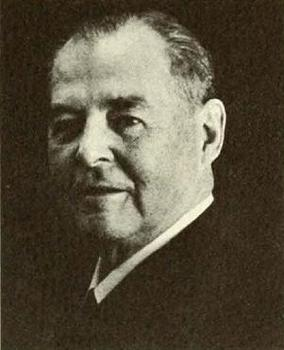
\includegraphics{images/hotelling.jpg}
\caption{Harold Hotelling}
\end{figure}
\end{column}

\begin{column}{0.48\textwidth}
The game I've described here is a version of a model originally
described by Harold Hotelling (1895-1973)
\end{column}
\end{columns}
\end{frame}

\begin{frame}{Feature Space}
\protect\hypertarget{feature-space}{}
\begin{itemize}
\tightlist
\item
  Hotelling was less interested in physical location than location in
  feature space.
\item
  He wanted an explanation of why the products of competing firms tended
  to be like one another.
\end{itemize}
\end{frame}

\begin{frame}{Political Versions}
\protect\hypertarget{political-versions}{}
\begin{itemize}
\tightlist
\item
  Games like this have become favorite tools of political scientists,
  arguing why political parties tended (at least in the 20th century!)
  to move towards the median.
\item
  You have to be careful about the payoffs here; political parties don't
  want to maximise votes, they want to maximise win probability and
  policy outcomes.
\item
  It turns out under a lot of assumptions you still get something like
  Hotelling's result, though it is sensitive to a lot of factors.
\end{itemize}
\end{frame}

\begin{frame}{Rationality Assumptions}
\protect\hypertarget{rationality-assumptions}{}
\begin{itemize}
\tightlist
\item
  Finally, I want to briefly flag the rationality assumptions this
  argument needs.
\item
  As long as the players are rational, they won't play 0/6.
\item
  As long as they know the other player is rational, they won't play
  1/5.
\item
  But to rule out 2/4, we need something stronger. We need that they
  each know that the other knows that each is rational.
\item
  For longer beaches, we need even stronger assumptions. And those
  assumptions may be implausible.
\end{itemize}
\end{frame}

\begin{frame}{For Next Time}
\protect\hypertarget{for-next-time}{}
\begin{itemize}
\tightlist
\item
  We will look at the most famous concept in game theory: Nash
  Equilibrium.
\end{itemize}
\end{frame}

\end{document}
